\documentclass[10pt]{beamer}

%%%
% PREAMBLE FOR THIS DOC 
%%%
%https://tex.stackexchange.com/questions/68821/is-it-possible-to-create-a-latex-preamble-header
\usepackage{/Users/miw267/Repos/csci246_spring2025/slides/preambles/beamer_preamble_for_CSCI246}


%%% TRY TO RESHOW TOC AT EACH SECTION START (with current section highlighted)
% Reference: https://tex.stackexchange.com/questions/280436/how-to-highlight-a-specific-section-in-beamer-toc
\newcommand\tocforsect[2]{%
  \begingroup
  \edef\safesection{\thesection}
  \setcounter{section}{#1}
  \tableofcontents[#2,currentsection]
  \setcounter{section}{\safesection}
  \endgroup
}


\usepackage[normalem]{ulem} % for strikeout (\sout)

%%%% HERES HOW TO DO IT CORRECTLY
% FIRST IN .STY FILE, DO
%\usetheme[sectionpage=none]{metropolis}
% THEN AT EACH SECTION DO
%\begin{frame}{Outline}
%  \tableofcontents[currentsection]	
%\end{frame}



%\setbeamertemplate{navigation symbols}{}
%\setbeamertemplate{footline}[frame number]{}


%%%
% DOCUMENT
%%%

\begin{document}

%\maketitle

%% Title page frame
%\begin{frame}
%    \titlepage 
%\end{frame}



\title{04/11/2025: Subgraphs}
\author{CSCI 246: Discrete Structures}
\date{Textbook reference: Sec 48, Scheinerman}

\begin{frame}
    \titlepage 
\end{frame}


\begin{frame}
\small
\begin{mygreenbox}[title=Graded Quiz Pickup]
Quizzes are in the front of the room, grouped into four bins (A-G, H-L, M-R, S-Z) by last name. The quizzes are upside down with your last name on the back. Come find yours before, during, or after class. Only turn the quiz over if it's yours.
\end{mygreenbox} 
\vfill 
%\begin{myredbox}[title=Friday's Problems Quiz]
%The problems quiz on Friday (04/02) will cover:
%\begin{itemize}
%\item Conditional Probability and Independence
%\item Random Variables
%\item Expectations	
%\end{itemize}
%
%\end{myredbox}
\vfill 
\begin{myyellowbox}[title=Today's Agenda]
\begin{itemize}
	\item Problems and reading quiz (15 mins)
	\item Mini-lecture ($\approx$ 10 mins)
	\item Group exercises ($\approx$ 20 mins)
\end{itemize}


\end{myyellowbox}
\vfill 

\end{frame}






\begin{frame}[standout]
Feedback on Wednesday's Quiz
\end{frame}


\begin{frame}{Reading Quiz Scores}
\begin{figure}[ht]
        \centering
        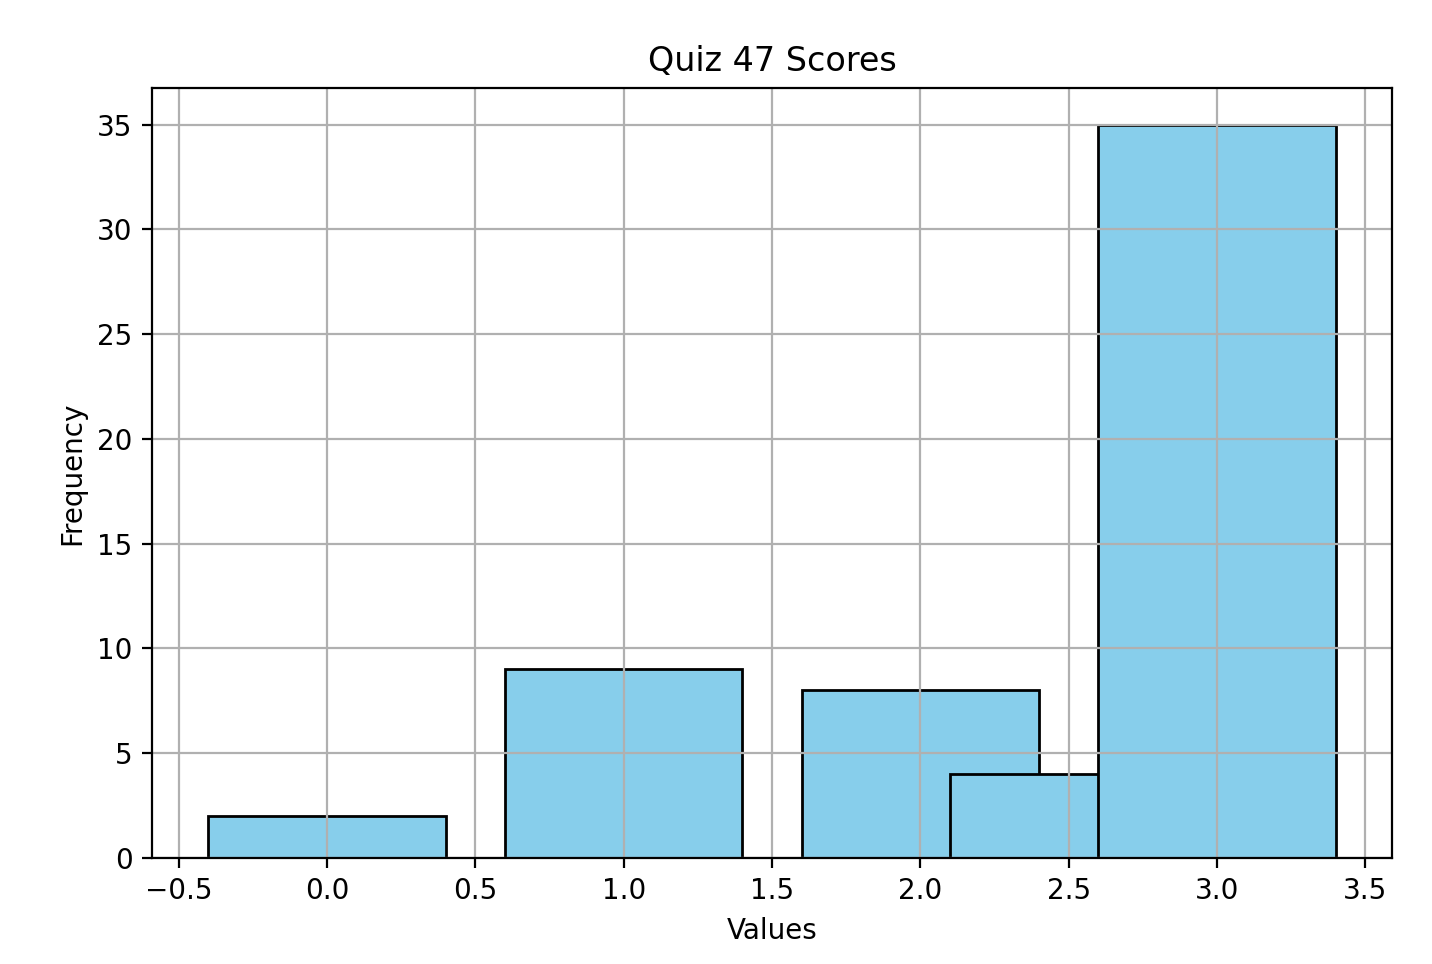
\includegraphics[width=.9\textwidth]{images/reading_quiz_scores}
   		 \caption{Median Score = 3/3 (100\%)}
\end{figure}
%\vfill 
%\textbf{Grading Rubric:}  
%\begin{enumerate}
%\item (1 point) Needed to give  reasonable answer to number of elementary operations (for the WHOLE algorithm snippet).
%\item (1 point) Stating the order (ideally as Big Theta, but Big O was accepted)
%\end{enumerate}


\end{frame}	




\begin{frame}[standout]
Today's quiz
\end{frame}

\begin{frame}
\small 

\begin{mygreenbox}[title=\text{Problems Quiz (recurrence, big O notation, algorithm efficiency)}]

\begin{enumerate}
\item Solve the recurrence relation $a_n = 4 a_{n-1} -4 a_{n-2}$  with initial conditions $a_0=5$ and $a_1=1$ to give an explicit formula for $a_n$. 
\item Let $a_n = 3n^2 + 7$. Prove that $a_n = \Theta (n^2)$.
\end{enumerate}
\end{mygreenbox}
\vfill 
\begin{myyellowbox}[title=\text{Reference material about second-order recurrences}]
To solve a recurrence of the form $a_n = s_1 a_{n-1} + s_2 a_{n-2}$, solve the quadratic formula $x^2 - s_1 x - s_2 =0$ to find roots $r_1$ and $r_2$. If $r_1 \neq r_2$, then $a_n = c_1 r_1^n + c_2 r_2^n$. If $r_1 = r_2 \defeq r$, then  $a_n = c_1 r^n + c_2 n r^n$. Then find $c_1$ and $c_2$.
\end{myyellowbox}


\vfill 
\begin{myredbox}[title=Reading Quiz (Subgraphs)]
Name one clique and one independent set from the graph below.
\begin{figure}
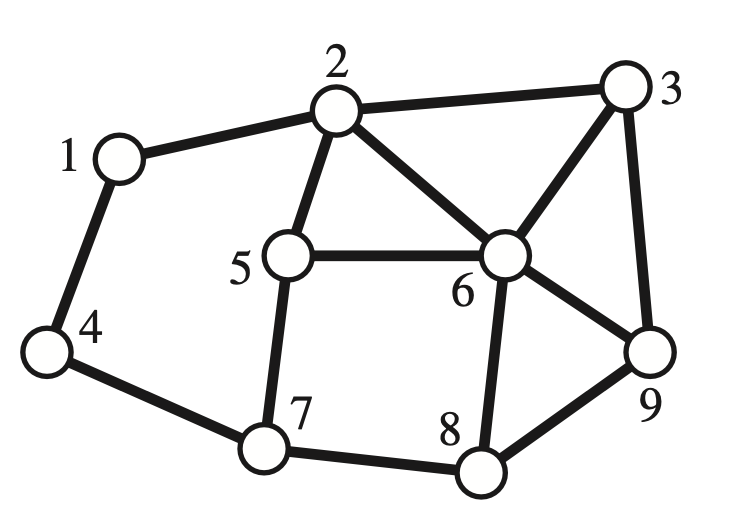
\includegraphics[width=.4\linewidth]{images/graph.png}
\end{figure}
\end{myredbox}
\end{frame}



\begin{frame}[standout]
Thoughts On Subgraphs
\end{frame}


\begin{frame}{Subgraphs}
\small 
\colorbox{yellow!30}{\textbf{Poll.}} How would you describe a \textbf{subgraph} in words?
\vfill
\pause 
\colorbox{green!30}{\textbf Definition.} Let $G$ and $H$ be graphs.  We call $G$ a \textbf{subgraph} of $H$ provided $V(G) \subseteq V(H)$ and $E(G) \subseteq E(H)$. 
\vfill 
\pause 
\begin{mygreenbox}[title=\text{Example: G is a \textbf{subgraph} of H}]
\begin{figure}
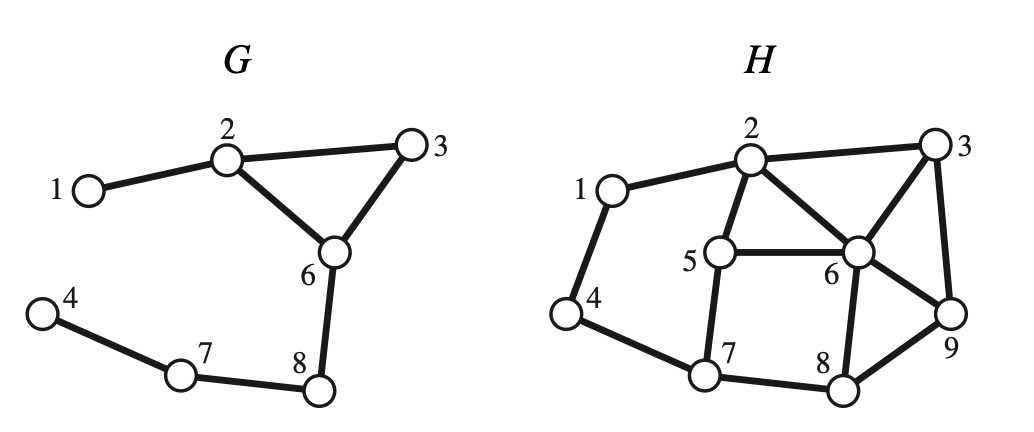
\includegraphics[width=\textwidth]{images/subgraph_general.png}
\end{figure}	
\end{mygreenbox}
\vfill 
\pause 
\colorbox{red!30}{\textbf{Solution.}} Possibly remove some vertices (and edges that touch them, so that you still have a graph).  Then possibly remove some additional edges.	
\end{frame}


\begin{frame}{Induced subgraphs}
\small 

\colorbox{yellow!30}{\textbf{Poll.}} How would you describe an \textbf{induced subgraph} in words?
\vfill
\pause 
\colorbox{green!30}{\textbf Definition.} Let $H$ be a graph and $A \subseteq V(H)$.  Then the subgraph of $H$ induced on $A$ is the graph $H[A]$ defined by
%
\begin{align*}
V(H[A]) &= A, \quad \text{and} \\
E(H[A]) &= \set{xy \in E(H) : x \in A \text{ and} y \in A}.	
\end{align*}

\vfill 
\pause 
\begin{mygreenbox}[title=\text{Example: G is an \textbf{induced subgraph} of H}]
\begin{figure}
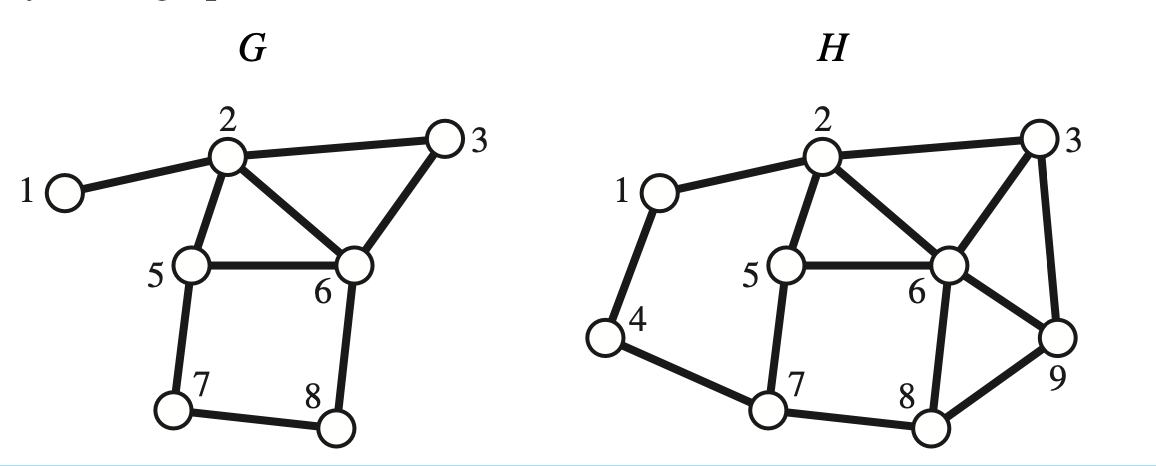
\includegraphics[width=.7\textwidth]{images/subgraph_induced.png}
\end{figure}	
\end{mygreenbox}
\vfill 
\pause 
\colorbox{red!30}{\textbf{Solution.}} Possibly remove some vertices (and edges that touch them, so that you still have a graph).  \textcolor{red}{\sout{Then possibly remove some additional edges.}}	
\end{frame}


\begin{frame}{Spanning subgraphs}


\colorbox{yellow!30}{\textbf{Poll.}} How would you describe a \textbf{spanning subgraph} in words?
\vfill 
\pause 

\colorbox{green!30}{\textbf Definition.} Let $G$ and $H$ be graphs.  We call $G$ a \textbf{spanning subgraph} of $H$ provided $G$ is a subgraph of $H$ and $V(G)=V(H)$.
\vfill
\pause 
\begin{mygreenbox}[title=\text{Example: G is a \textbf{spanning subgraph} of H}]
\begin{figure}
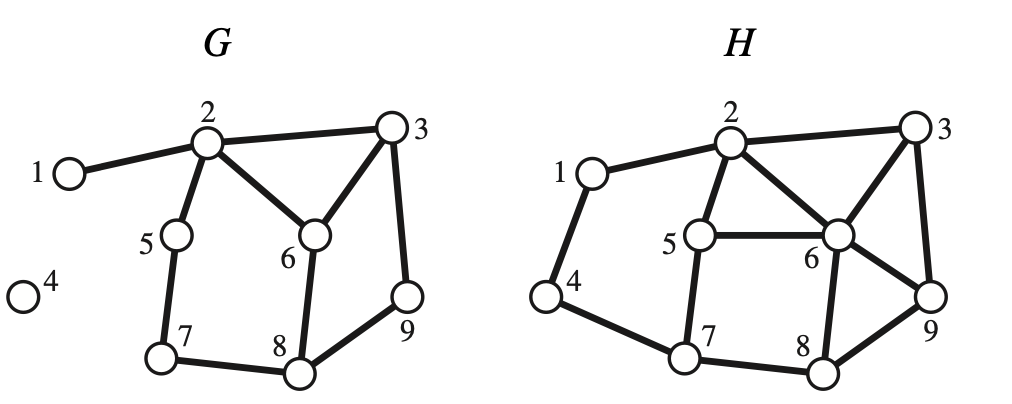
\includegraphics[width=.8\textwidth]{images/subgraph_spanning.png}
\end{figure}	
\end{mygreenbox}
\vfill 
\pause 
\colorbox{red!30}{\textbf{Solution.}} \textcolor{red}{\sout{ Possibly remove some vertices (and edges that touch them, so that you still have a graph). Then}}	 possibly remove some \textcolor{red}{\sout{additional}} edges.
\end{frame}


\begin{frame}[standout]
Group exercises
\end{frame}

\begin{frame}
\footnotesize 
\vfill 
\begin{columns}
\begin{column}{0.33\textwidth}
aaron.loomis: 18 \\ 
adam.wyszynski: 4 \\ 
alexander.knutson: 2 \\ 
anthony.mann: 3 \\ 
blake.leone: 8 \\ 
bridger.voss: 5 \\ 
caitlin.hermanson: 3 \\ 
cameron.wittrock: 20 \\ 
carsten.brooks: 5 \\ 
carver.wambold: 10 \\ 
colter.huber: 6 \\ 
conner.reed1: 12 \\ 
connor.mizner: 11 \\ 
connor.yetter: 20 \\ 
derek.price4: 6 \\ 
devon.maurer: 8 \\ 
emmeri.grooms: 1 \\ 
erik.moore3: 12 \\ 
ethan.johnson18: 10 \\ 
evan.barth: 4 \\ 
evan.schoening: 19 \\\end{column}
\begin{column}{0.33\textwidth}
griffin.short: 9 \\ 
jack.fry: 8 \\ 
jacob.ketola: 6 \\ 
jacob.shepherd1: 14 \\ 
jada.zorn: 1 \\ 
jakob.kominsky: 14 \\ 
james.brubaker: 19 \\ 
jeremiah.mackey: 14 \\ 
jett.girard: 16 \\ 
john.fotheringham: 4 \\ 
jonas.zeiler: 1 \\ 
joseph.mergenthaler: 15 \\ 
joseph.triem: 9 \\ 
julia.larsen: 13 \\ 
justice.mosso: 18 \\ 
kaden.price: 11 \\ 
lucas.jones6: 2 \\ 
luka.derry: 16 \\ 
luke.donaldson1: 9 \\\end{column}
\begin{column}{0.33\textwidth}
lynsey.read: 16 \\ 
mason.barnocky: 20 \\ 
matthew.nagel: 2 \\ 
micaylyn.parker: 7 \\ 
michael.oswald: 19 \\ 
nolan.scott1: 13 \\ 
owen.obrien: 18 \\ 
pendleton.johnston: 13 \\ 
peter.buckley1: 17 \\ 
reid.pickert: 3 \\ 
ryan.barrett2: 15 \\ 
samuel.hemmen: 10 \\ 
samuel.mosier: 11 \\ 
samuel.rollins: 16 \\ 
sarah.periolat: 5 \\ 
timothy.true: 17 \\ 
tristan.nogacki: 12 \\ 
tyler.broesel: 7 \\ 
william.elder1: 15 \\ 
yebin.wallace: 7 \\ 
zeke.baumann: 17 \\\end{column}
\end{columns}
\vfill
\end{frame}

\begin{frame}{Group exercises}
\small 
\noindent
\begin{minipage}[c]{0.6\textwidth}
\begin{enumerate}
	\item  Let $G$ be the graph in the top figure.   Draw pictures of the following subgraphs: (a) $G-1$, (b) $G-\set{5,6}$, (c) $G[\set{3,4,6}]$, (d) $G[\set{2,4,6}]$.
	\item Which of the various properties of relations does the is-a-subgraph-of relation exhibit? Is it reflexive? Symmetric? Transitive?
    \item Let $G$ be a complete graph with $n$ vertices.  (a) How many spanning subgraphs does $G$ have? (b) How many induced subgraphs does $G$ have?
    \item Let $G$ and $H$ be the two graphs in the bottom figure.  Please find $\alpha(G), \omega(G), \alpha(H), \omega(H)$.  (Recall that $\alpha(\cdot)$ is the size of a largest independent set and $\omega(\cdot)$ is the size of a largest clique.) 
\end{enumerate}
\end{minipage}%
\hfill
\begin{minipage}[c]{0.38\textwidth}
   
    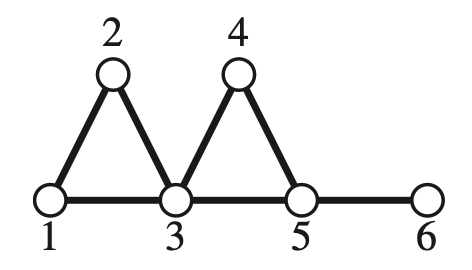
\includegraphics[width=\textwidth]{images/subgraph_1} %
    
    \vspace{4cm}
    
    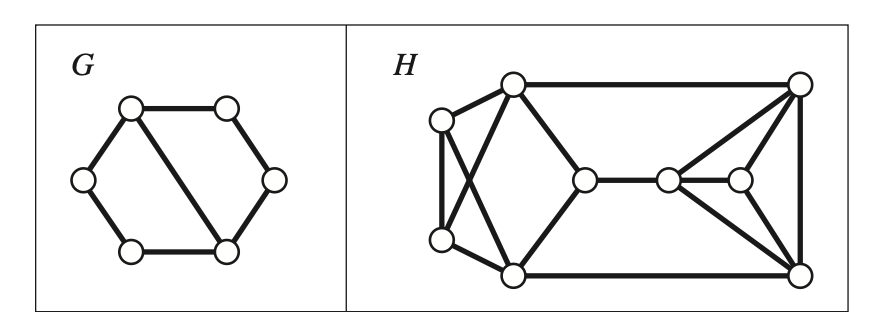
\includegraphics[width=\textwidth]{images/subgraph_2}
\end{minipage}%    

\end{frame}


\begin{frame}{Solution to group exercise \#1a}
\small 
\textbf{Problem.} Let $G$ be the graph in the figure below.   Draw a picture of the subgraph $G-1$. 
\vfill 
\begin{center}
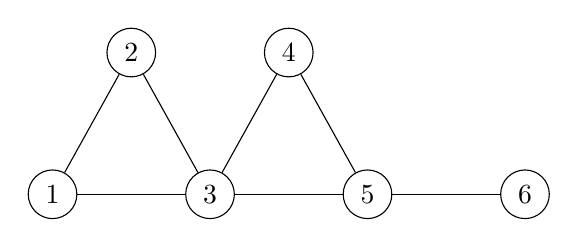
\begin{tikzpicture}[every node/.style={circle, draw, minimum size=0.5cm}, node distance=2cm]

    % Bottom row
    \node (1) at (0,0) {1};
    \node (3) at (2,0) {3};
    \node (5) at (4,0) {5};
    \node (6) at (6,0) {6};

    % Top row
    \node (2) at (1,1.8) {2}; % centered above B1 and B2
    \node (4) at (3,1.8) {4}; % centered above B3 and B4

    % Edges
    \draw (2) -- (1);
    \draw (2) -- (3);
    \draw (4) -- (3);
    \draw (4) -- (5);
    \draw (1) -- (3);
    \draw (3) -- (5);
    \draw (5) -- (6);

\end{tikzpicture}
\end{center}

\vfill 
\textbf{Solution.} \\[1ex]
\centering
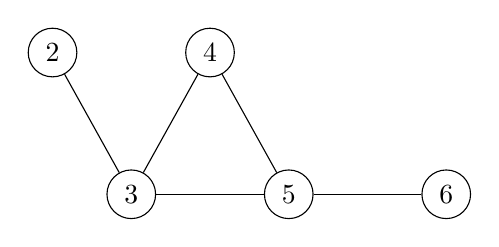
\begin{tikzpicture}[every node/.style={circle, draw, minimum size=0.5cm}, node distance=2cm]

    % Bottom row
    \node (3) at (2,0) {3};
    \node (5) at (4,0) {5};
    \node (6) at (6,0) {6};

    % Top row
    \node (2) at (1,1.8) {2}; % centered above B1 and B2
    \node (4) at (3,1.8) {4}; % centered above B3 and B4

    % Edges
    \draw (2) -- (3);
    \draw (4) -- (3);
    \draw (4) -- (5);
    \draw (3) -- (5);
    \draw (5) -- (6);

\end{tikzpicture}


\end{frame}


\begin{frame}{Solution to group exercise \#1b}
\small 
\textbf{Problem.} Let $G$ be the graph in the figure below.   Draw a picture of the subgraph $G-\set{5,6}$. 
\vfill 
\begin{center}
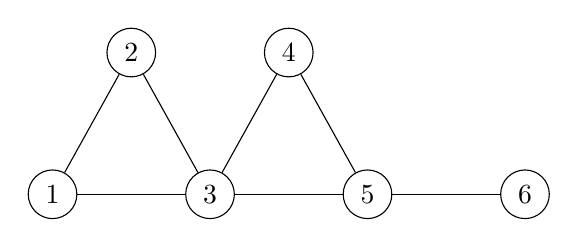
\begin{tikzpicture}[every node/.style={circle, draw, minimum size=0.5cm}, node distance=2cm]

    % Bottom row
    \node (1) at (0,0) {1};
    \node (3) at (2,0) {3};
    \node (5) at (4,0) {5};
    \node (6) at (6,0) {6};

    % Top row
    \node (2) at (1,1.8) {2}; % centered above B1 and B2
    \node (4) at (3,1.8) {4}; % centered above B3 and B4

    % Edges
    \draw (2) -- (1);
    \draw (2) -- (3);
    \draw (4) -- (3);
    \draw (4) -- (5);
    \draw (1) -- (3);
    \draw (3) -- (5);
    \draw (5) -- (6);

\end{tikzpicture}
\end{center}

\vfill 
\textbf{Solution.} \\[1ex]
\begin{center}
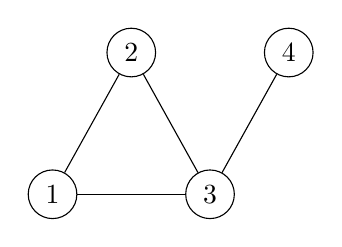
\begin{tikzpicture}[every node/.style={circle, draw, minimum size=0.5cm}, node distance=2cm]

    % Bottom row
    \node (1) at (0,0) {1};
    \node (3) at (2,0) {3};

    % Top row
    \node (2) at (1,1.8) {2}; % centered above B1 and B2
    \node (4) at (3,1.8) {4}; % centered above B3 and B4

    % Edges
    \draw (2) -- (1);
    \draw (2) -- (3);
    \draw (4) -- (3);
    \draw (1) -- (3);

\end{tikzpicture}
\end{center}

\end{frame}


\begin{frame}{Solution to group exercise \#1c}
\small 
\textbf{Problem.} Let $G$ be the graph in the figure below.   Draw a picture of the subgraph $G[\set{3,4,6}]$. 
\vfill 
\begin{center}
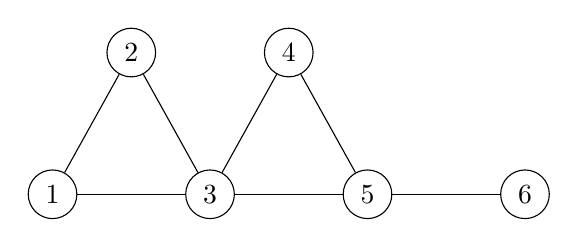
\begin{tikzpicture}[every node/.style={circle, draw, minimum size=0.5cm}, node distance=2cm]

    % Bottom row
    \node (1) at (0,0) {1};
    \node (3) at (2,0) {3};
    \node (5) at (4,0) {5};
    \node (6) at (6,0) {6};

    % Top row
    \node (2) at (1,1.8) {2}; % centered above B1 and B2
    \node (4) at (3,1.8) {4}; % centered above B3 and B4

    % Edges
    \draw (2) -- (1);
    \draw (2) -- (3);
    \draw (4) -- (3);
    \draw (4) -- (5);
    \draw (1) -- (3);
    \draw (3) -- (5);
    \draw (5) -- (6);

\end{tikzpicture}
\end{center}

\vfill 
\textbf{Solution.} \\[1ex]
\begin{center}
\begin{tikzpicture}[every node/.style={circle, draw, minimum size=0.5cm}, node distance=2cm]

    % Bottom row
    \node (3) at (2,0) {3};
    \node (6) at (6,0) {6};

    % Top row
    \node (4) at (3,1.8) {4}; % centered above B3 and B4

    % Edges
    \draw (4) -- (3);

\end{tikzpicture}
\end{center}

\end{frame}

\begin{frame}{Solution to group exercise \#1d}
\small 
\textbf{Problem.} Let $G$ be the graph in the figure below.   Draw a picture of the subgraph $G[\set{2,4,6}]$. 
\vfill 
\begin{center}
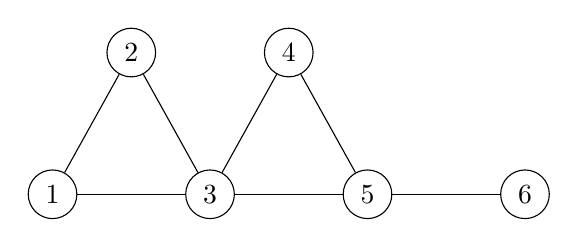
\begin{tikzpicture}[every node/.style={circle, draw, minimum size=0.5cm}, node distance=2cm]

    % Bottom row
    \node (1) at (0,0) {1};
    \node (3) at (2,0) {3};
    \node (5) at (4,0) {5};
    \node (6) at (6,0) {6};

    % Top row
    \node (2) at (1,1.8) {2}; % centered above B1 and B2
    \node (4) at (3,1.8) {4}; % centered above B3 and B4

    % Edges
    \draw (2) -- (1);
    \draw (2) -- (3);
    \draw (4) -- (3);
    \draw (4) -- (5);
    \draw (1) -- (3);
    \draw (3) -- (5);
    \draw (5) -- (6);

\end{tikzpicture}
\end{center}

\vfill 
\textbf{Solution.} \\[1ex]
\begin{center}
\begin{tikzpicture}[every node/.style={circle, draw, minimum size=0.5cm}, node distance=2cm]

    % Bottom row
    \node (6) at (6,0) {6};

    % Top row
    \node (2) at (1,1.8) {2}; % centered above B1 and B2
    \node (4) at (3,1.8) {4}; % centered above B3 and B4


\end{tikzpicture}
\end{center}
\end{frame}

\begin{frame}{Solution to group exercise \#2}
\textbf{Problem.} Which of the various properties of relations does the is-a-subgraph-of relation exhibit? Is it reflexive? Symmetric? Transitive?
\vfill

\textbf{Solution.}
\begin{itemize}
\item \textbf{Reflexive?} Yes, $G=(V,E)$ is a subgraph of itself, since $V \subseteq V$ and 	$E \subseteq E$.
\item  \textbf{Symmetric?} No. Let $G=(V_G, E_G)$ be a subgraph of $H=(V_H,E_H)$ where either $V_G \subsetneq V_H$ or $E_G \subsetneq E_H$.  In the first case, $V_H \subseteq V_G$ fails, and in the second case  $E_H \subseteq E_G$ fails.  Either way, $G$ is not a subgraph of $H$.
\item \textbf{Transitive?} Yes. Let $F=(V_F, E_F)$ be a subgraph of  $G=(V_G, E_G)$ and  $G$ be a subgraph of  $H=(V_H, E_H)$.   Then $V_F \subseteq V_G \subseteq V_H$ and  $E_F \subseteq E_G \subseteq E_H$  by definition of subgraph (and transitivity of the subset operation).  In particular, $V_F \subseteq V_H$ and  $E_F \subseteq E_H$. Hence $F$ is a subgraph of $H$.
\end{itemize}
	
\end{frame}

\begin{frame}{Solution to group exercise \#3}
\small 
\textbf{Problem.} Let $G$ be a complete graph with $n$ vertices.  (a) How many spanning subgraphs does $G$ have? (b) How many induced subgraphs does $G$ have?
\vfill

\textbf{Solution.}
\begin{itemize}
\item[(a).] The solution is $2^{\binom{n}{2}}$.  A complete graph with $n$ vertices has $\binom{n}{2}=\frac{n(n-1)}{2}$ edges (since there are $\binom{n}{2}$ ways to choose pairs from a set of $n$ items).  A spanning subgraph keeps all the original vertices and deletes some number of the edges (possibly none, possibly all).  In other words, for each edge, we make a free binary decision to keep or delete the edge.  Thus, there are $2^{\binom{n}{2}}$ possible spanning subgraphs.  (Note that the conclusion can be justified via Scheinerman Theorem 8.6, if we imagine forming a list of length $\binom{n}{2}$, where each element of the list is chosen from a pool of 2 choices.)
\item[(b).] There are $2^n$ different ways to form subsets of $n$ vertices.  Each subset determines an induced subgraph (since an induced subgraph is determined by keeping a subset of vertices, and then removing exactly the edges that touch at least one vertex that has been discarded.)  Hence, there are $2^n$ possible induced subgraphs of $G$. (Note that this argument applies to any graph $G$ with $n$ vertices, not just complete graphs.)
\end{itemize}

\end{frame}


\begin{frame}{Solution to group exercise \#4}
\small 
\textbf{Problem.}   Let $G$ and $H$ be the two graphs in the figure below.  Please find $\alpha(G), \omega(G), \alpha(H), \omega(H)$.  (Recall that $\alpha(\cdot)$ is the size of a largest independent set and $\omega(\cdot)$ is the size of a largest clique.) 
   
\begin{figure}
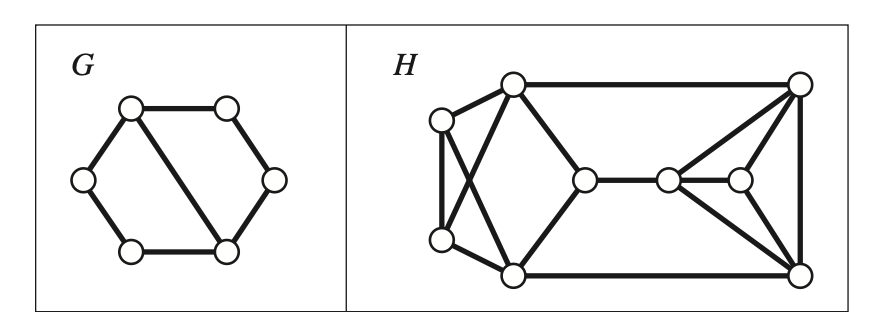
\includegraphics[width=.5\textwidth]{images/subgraph_2} %	
\end{figure}
\vfill 
\textbf{Solution.}
%
\[ \omega(G)=2, \quad \alpha(G)=3, \quad  \omega(H)=3\,?, \quad  \alpha(H)=??? \]
%
The main point of this exercise is that it's annoying to try to compute these by brute force as the number of vertices $n$ grows. For example, to find a brute force solution for $\alpha(\cdot)$, you would need to try all subsets of vertices and check which are independent. However,  this procedure has time complexity $O(2^n)$, so it is only practical for small graphs.  Further study of graph theory would introduce algorithms to compute these quantities. 
\end{frame} 

\end{document}
